\documentclass[11pt,a4paper]{article}

\usepackage[T1]{fontenc}
\usepackage[utf8]{inputenc}
\usepackage[frenchb]{babel} % Global stuff set to french
\usepackage[margin=2.5cm]{geometry} % The margin of the page
%\usepackage{amsmath}  % to include math formulas
\usepackage{graphicx} % to include pictures
\usepackage[hidelinks]{hyperref} % To include hyperlinks in a PDF
\usepackage{fancyhdr} % to be able to make the page fancy looking
\usepackage{lastpage} % so latex knows what is the last page...
\usepackage{appendix} % To make appendixes
\usepackage{color} % For text colors
\usepackage{palatino} % Change font
%\usepackage{tabularx}
\usepackage{changepage}
\usepackage{subcaption}
\usepackage{enumitem}

%% Fancy layout
\pagestyle{fancy}
    \lhead{Projet d'année - Partie 1}
    \chead{}
    \rhead{Groupe 2}
    \lfoot{}
    \cfoot{}
    \rfoot{Page \thepage\ de \pageref{LastPage}}
\renewcommand{\headrulewidth}{0.4pt}
\renewcommand{\footrulewidth}{0.4pt}


%%% --- %%% --- DOCUMENT START --- %%% --- %%%
\begin{document}
    \begin{titlepage}

\topskip0pt
\begin{center}
    \vspace*{\fill}
        \hrule
        \vspace*{2pt}
        \hrule
        \vspace*{15pt}
        \textsc{\Huge{INFO-F106 : Projet d'année \\\vspace*{8pt} Rappport intermédiaire}}
        \vspace*{15pt}
        \hrule
        \vspace*{2pt}
        \hrule
  \vspace*{\fill}
\end{center}
\null
\vfill
  
\large{Mardi 16 décembre 2014} \hfill \large{Carlos Requena López - \emph{410031}}

\end{titlepage}
    \pagestyle{empty}
\tableofcontents
\newpage
 %%% Counting pages now %%%
\pagestyle{fancy}

\setcounter{page}{1}

\section{Introduction}
\label{sec:intro}

\subsection{But du projet}
\label{sec:but}

Dans le cadre du projet d'analyse et méthode et de système d'exploitation, il est demandé d'implémenter un jeu de carte en ligne basé sur une architecture client/serveur en C/C++.
\medbreak
Ce projet devra fournir un jeu de carte symétrique où deux joueurs pourront s'affronter et gagner des points pour un classement général. Chaque joueur disposera d'une collection de cartes à partir de laquelle il pourra construire des decks. Ces decks contiendront des cartes de type créature qui peuvent attaquer et des cartes de type sort qui lanceront des événements spéciaux.
\medbreak
Le projet requière la mise en place d'une architectures client/serveur avec le client qui sert principalement d'interface de jeu (graphique ou console) et les calculs qui seront effectué côté serveur. Il est donc important de développer un serveur robuste, efficace et rapide qui soit en mesure de gérer plusieures parties simultanément tout en fournissant des services tels que le classement général, un service de compte et de login ainsi qu'un service de messagerie instantané entre deux joueurs. Pour cela, nous seront ammené à développer une application capable de gérer un maximum de cas de figure pour garantir la continuité et la stabilité de ces différent services. La gestion d'erreurs devra être telle que cette erreur ne perturbera aucune autre partie ni aucun des autres services.
\medbreak
Le Wizard Poker sera disponible à n'importe quel joueurs enregistré pour jouer contre d'autre joueurs et essayer de gagner des places dans le calssement générale. Il permetra aussi à de nouveau joueurs de consulter ce classement et de s'enregistrer en tant que nouveau joueur. Dans ce cas, le joueurs recevra ses premières cartes et sera invité à confectionner son premier deck avant d'affronter son premier adversaire.

% Texte (d’une demi-page approximativement) décrivant les tenants et
% aboutissants du projet, et énumérant les différents types de
% personnes qui vont bénéficier de la réalisation du projet.

\subsection{Glossaire}
\label{sec:glo}

% Définition des termes, des acronymes et des abréviations utilisés
% dans le présent document.

\begin{itemize}
\item \textbf{Deck:} Collection de 20 cartes qui...
\end{itemize}

\subsection{Historique du document}
\label{sec:hist}

% Tableau reprenant tous les changements effectués sur le
% document. Chaque ligne de celui-ci contiendra les champs suivants :
% numéro de version, auteur et date de la modification, description
% des changements. Le tableau sera trié de manière décroissante sur le
% numéro de version.

% Example de versioning:


    % 0 for alpha (status)
    % 1 for beta (status)
    % 2 for release candidate
    % 3 for (final) release


\begin{table}[h]
  \centering
  \begin{tabular}[ht]{|l|l|l|p{18em}|}
    \hline

    \textbf{Version}
    & \textbf{Auteur}
    & \textbf{Date modification}
    & \textbf{Description des changements}\\ \hline \hline
    NEXT &  &  &  \\ \hline
    NEXT &  &  &  \\ \hline
    v0.0 & Carlos Requena & 26/11/15 22:30
    & Mis en place. Diagrammes realisés en groupe le 25/11/15 ajoutés\\ \hline
  \end{tabular}
  \caption{Changements document}
  \label{tab:hist}
\end{table}

\section{Besoins de l'utilisateur}
\label{sec:besoins}

% Cette deuxième section reprend les services que le système doit
% fournir aux utilisateurs, ainsi que les contraintes de
% fonctionnement du système. Elle doit être complète et consistante,
% et il faut qu’elle soit rédigée dans un langage spécialement
% compréhensible pour le client, c’est-à-dire en évitant entre autres
% tout terme ou détail techniques.

\subsection{Exigences fonctionnelles}
\label{sec:exi-fonc}

% Ce type d’exigences sera décrit en utilisant des diagrammes use case
% et en fournissant une description pour chacun d’entre eux (comme vu
% au cours théorique et aux exercices).

\subsection{Exigences non fonctionnelles}
\label{sec:exi-nonfonc}



\subsection{Exigences de domaine}
\label{sec:exi-dom}

\section{Besoins du systeme}
\label{sec:besoins-sys}

% Cette troisième section décrit en détail les fonctionnalités du
% système (à partir de celles décrites à la section précédente), sans
% aborder (dans la mesure du possible) *comment* elles doivent être
% réalisées.

\subsection{Exigences fonctionnelles}
\label{sec:exi-fonc-sys}

% Ce type d’exigences sera décrit en utilisant des diagrammes use
% case et en fournissant une description *plus détaillée* pour
% chacun d’entre eux (comme vu au cours théorique et aux exercices).

Sequence diagram pour interaction??

Le système doit interagir avec l'utilisateur, et lui proposer certaines actions, comme commencer un duel, gérer ses decks, consulter le classement des joueurs, etc.

Pour les nouveaux joueurs, l'application doit offrir la possibilité de s'enregistrer, avec un pseudonyme et un mot de passe.


\subsection{Exigences non fonctionnelles}
\label{sec:exi-nonfonc-sys}

Les exigences non fonctionnelles décrivent le comportement de l'application.

Le système doit être tout d'abord robuste et stable, c'est-à-dire gérer les erreurs et éviter les crashs et les déconnexions... Il doit par ailleurs être agréable d'utilisation pour l'utilisateur (ergonomie et esthétique/design) et garantir que celui-ci ne puisse pas tricher pendant une partie.

Donc en résumé, robuste, stable, sûr, et excessivement amusant. Des heures de franche rigolade, en toute sécurité, sont assurées à tout utilisateur du jeu.

\subsection{Design et fonctionnement du systeme}
\label{sec:design}

% Cette partie sera décrite à l’aide des différents diagrammes UML
% vus au cours théorique et aux exercices.

\begin{figure}[ht]
  \centering
  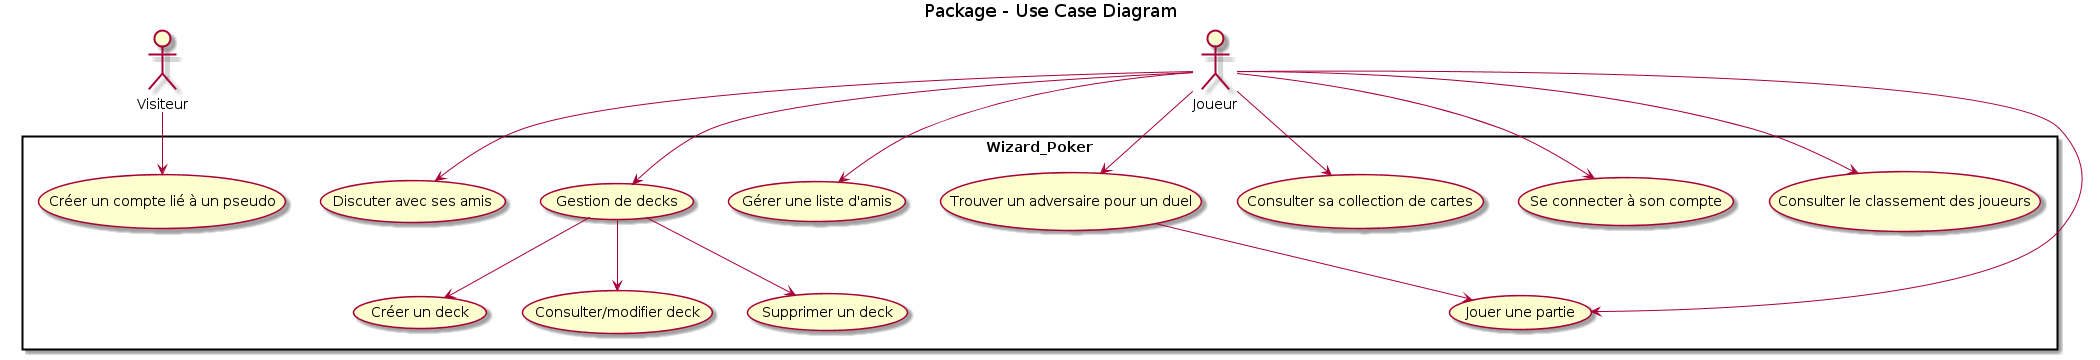
\includegraphics[width=1\textwidth]{uml_files/UseCaseDiagram.png}
  \caption{\label{fig:usecase} Use Case Diagram du jeu en question}
\end{figure}

\begin{figure}[ht]
  \centering
  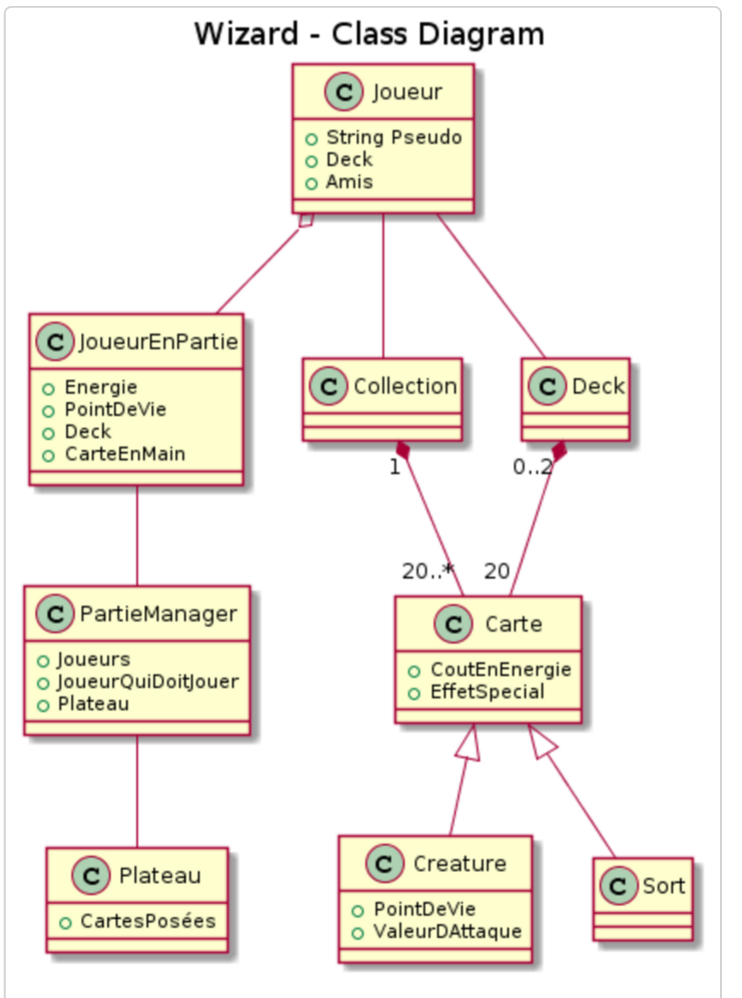
\includegraphics[width=1\textwidth]{uml_files/ClassDiagram.png}
  \caption{\label{fig:class} Diagramme des classes}
\end{figure}


\appendix

\section{Index des termes utilisés}
\label{sec:index}

\end{document}
